\chapter[Place naming strategies in Lower Tanana Dene (Athabascan)]{\vspace{-125pt}
{\normalfont\normalsize\begin{flushright}\textit{``People used to name these things as they see them.''}\\[2pt]--Chief Peter John\\\end{flushright}\bigskip\bigskip
% {\normalfont\normalsize
%\hspace{0.2\textwidth}\parbox{0.8\textwidth}{
% \textit{``People used to name these things as they see them.''
%}\\[2pt] \strut\hfill (Chief Peter John)\\\bigskip
%\hspace{0.2\textwidth}\parbox{0.8\textwidth}{In Athabascan country, ``a bear den is sometimes named after the hunter who found it.''
%}\\[2pt] \strut\hfill\citep[244]{nelson1982}}\\\bigskip}
}
Place naming strategies in Lower Tanana Dene (Athabascan)}

\sethandle{10125/24844}

%\def\authorlast{Holton \& Harris}
\def\authorlast{Harris \& Holton}

\renewcommand{\beginchapter}{\pageref{holton-ch-begin}}
\renewcommand{\finishchapter}{\pageref{holton-ch-end}}
\label{holton-ch-begin}
\thispagestyle{firststyle}

%\chapauth{Gary Holton}
%\affiliation{University of Hawai‘i at Mānoa}
%\chapauth{David Jason Harris}
%\affiliation{University of Alaska Fairbanks}
%\authortoc{Gary Holton \& David Jason Harris}

\chapauth{David Jason Harris}
\affiliation{University of Alaska Fairbanks}
\chapauth{Gary Holton}
\affiliation{University of Hawai‘i at Mānoa}
\authortoc{David Jason Harris \& Gary Holton}


\begin{Abstract}\vspace{-5pt}
Like other Alaska Dene languages, Lower Tanana employs a “generative” place naming strategy in which a specific term combines with one of a closed set of landscape generic terms to create a binomial name. However, an empirical study of place naming strategies reveals that the generative strategy is rather exceptional: most Lower Tanana names do not exhibit a binomial generative structure. Moreover, the existence of a generative strategy fails to explain the choice of specific term. We hypothesize instead that place naming in Lower Tanana is primarily driven by human affordance, and we propose a tentative typology of place naming strategies.
\end{Abstract}


\section{Introduction}\hspace{-0.3cm}\footnote{\hl{Acknowledgements}. The Lower Tanana orthography used here follows \citet{kari2012}. \ortho{kh} represents the voiceless velar fricative, and \ortho{w} represents a mid-back vowel.}
One of Jim Kari’s seminal contributions to Dene ethnogeography is the recognition of what he has dubbed the Dene “generative geography capacity” \citep{kari2010}. This pattern is capable of generating multiple bi- or tri-nominal names consisting of a single shared specific term compounded with various generic landscape or directional terms. For example, the Lower Tanana names \textit{Sresr No’} and \textit{Sresr Bene’} are both binomial names which combine the specific term \textit{sresr} ‘black bear’ with the landscape generics \textit{no’} `stream’ and \textit{bene’}  ‘lake’, respectively, to derive two distinct place names in the same general area. The generative capacity in Dene naming is not only a tool for creating names but also a constraint on possible names. The constraining effects can be seen in the apparent predictability of Dene generative names.

While we can’t know in advance that a particular lake is named \textit{Sresr Bene’}, it is the case that \textit{Sresr Bene’} will likely be located in the vicinity of \textit{Sresr No’}---most likely a lake into which or out of which the stream known as \textit{Sresr No’} flows. While the location of the lake referenced by the name \textit{Sresr Bene’} in this example may not be precisely determined, certain landscape generics apparently leave little room for indeterminacy in location. For example, the generic \textit{chaget} ‘river mouth’ almost invariably references a location at the mouth of a stream, so that \textit{Sresr Chaget} would be located at the mouth of the stream \textit{Sresr No’}. The name \textit{Sresr Chaget} might refer to a specific location at the mouth of the river, or it may refer to the entire river mouth area in general, or it might refer to either depending on context. But in all cases the location of \textit{Sresr Chaget} is well-defined in relation to the stream \textit{Sresr No’}. Moreover, while we cannot know a priori that a particular location at a river mouth has a name, if it does have a name then it is likely to be \textit{Sresr Chaget}. It is as if a speaker already knows the name \textit{Sresr Chaget} before she even hears the name.

% this paragraph seems orphaned now 
%\hl{The prominence of the term \textit{chaget} and its cognates (from Proto-Dene *kæq’e) in Dene place names is evidenced in the large number of English names for Alaskan villages which derive from names including this term. Examples include: Crossjacket (from Lower Tanana \textit{K’osr Chaget}); Allakaket (from Koyukon \textit{Aalaa Kkaakk’et}); and Chalkyitsik (from Gwich’in \textit{ Jałgiitsik}).}

The generative capacity within Dene is usually demonstrated by citing elaborate examples of certain specific terms which admit multiple binomial generative names. For example, \citet{kari2008} notes that the Ahtna specific term \textit{Yidateni} occurs as a part of a cluster of ten distinct binomial and trinomial names. These examples are quite striking and clearly demonstrate the limits of what is possible in terms of generative naming in Dene languages. In this paper we taking a somewhat different approach to understanding generative naming. Rather than focusing on the most exotic examples of generative naming we instead attempt to situate the generative naming strategy within a broader suite of Dene place-naming strategies. We take a quantitativ	e approach, drawing on a comprehensive inventory Lower Tanana Dene place names. The list of names  used for this study contains 1063 names derived from the list published in  \citet{kari2012}. Our list is slightly shorter than the over 1080 names in the published list because we discarded several inadvertent duplicates as well as several English names for which no Lower Tanana name has been documented. Among the latter is the English name Salmonfoot Creek, which may well be a calque of a Lower Tanana name, though no Lower Tanana  name has been recovered. We also discarded unverified names from early sources, such as Chaytaltic, a name referred to by \citet{mcmanus1900} but which is not recognized by Lower Tanana speakers today.

While an analysis of the names themselves can reveal the presence of generative naming structures, these data are not always sufficient to determine place-naming strategies. Thus, we supplemented our study of the Lower Tanana place names list with a review of original speaker interviews conducted as part of a 1979 survey of place names in the Lower Tanana region \citep{andrews1980}. The original recordings, housed at the Alaska Native Language Archive, comprise roughly 20 hours of interviews conducted in both English and Dene. Based on an empirical analysis of 20 legacy recordings of place name interviews. These recordings were carefully annotated to by one of us (Harris) to identify place name descriptions and discussions of the motivations for particular place names.



\section{Preliminaries}
Before proceeding to discuss our classification of place-naming strategies, we first review two potentially confounding issues: predictability of names and duplication of names. It is important to distinguish generativity from predictability.


\subsection{Generative names and predictability}
Given the prominence of the generative pattern in Dene it is tempting to think that we already know the names of these places even before we learn them, but this begs the question of what it means to be a name. At the very least a place is named because speakers give it that name. Naming is a deliberate act, so not every mountain or lake or river mouth will have a name. Thus, term generative is slightly misleading when applied to Dene place-naming. The generative pattern creates possible names; actual names are constrained by what people choose to name. A more accurate way to state the generative claim is to say that if a feature is named, then it will be named using the appropriate landscape generic for that feature combined with a relevant specific term for the region. In the case of the river mouth feature in Lower Tanana the claim then would be that if a river mouth is named, then it will be named using the landscape generic \textit{chaget} combined with the specific term occurring in the name of the stream associated with that river mouth. 

There are several problems even with this more conservative formulation of the generative claim. First of all, river mouths do not always occur where we might think they do. That is, places whose names include the Lower Tanana generic term for ‘river mouth’ are not necessarily located at the mouths of rivers. A prominent example of this is the place known as \textit{Dradlaya Chaget,} which is located at the base of a hill where the Chatanika River (\textit{Dradlaya Nik’a}) flows west into the Minto Flats region \citep[see][]{holton2011c}. There is no mouth here in the traditional sense of a stream emptying into another river body, though there is a rather abrupt geomorphic change as the Chatanika leaves the hills and begins to flow through flatter terrain. The problem is that such geomorphic transitions happen repeatedly throughout Lower Tanana country without being designated using a name with \textit{chaget} ‘river mouth’. As noted above, places are named for a reason, and \textit{Dradlaya Chaget} is no exception. Peter John describes this place as the site of an old fish camp (ANLC0984a, 23:49, 1979-05-04).\footnote{Place name recordings are cited using their Alaska Native Language Archive identifier, followed by a time code, followed by date. See \url{http://www.uaf.edu/anla}}. Speakers chose to call this camp \textit{Dradlaya Chaget}, but crucially they didn’t have to call it this. They could have chosen a different name. In other words, the generative naming system is not entirely deterministic or predictable.

Further evidence for the lack of predictability in generative naming comes from the way in which the binomial names are constructed. In the cases of generative names we have discussed so far the generic term alternates in each name. Another example would be the pair \textit{Deltsedza No’} ‘mouse river’ and \textit{Deltsedza Ddhela’} `mouse mountain’, where the landscape generics \textit{no’} and \textit{ddhela’} generate two different names. In other cases one of the generic is retained in multiple names, and additional generics are compounded, as in the pair \textit{Nechuyh No’}  ‘rosehip stream’ and \textit{Nechuyh No’ Ddhela’} ‘rosehip stream mountain’. While this latter pattern is clearly generative in the sense that a landscape generic is used to generate another name, we have no way to predict whether the generated name will compound the additional generic, as in the attested name \textit{Nechuyh No’ Ddhela’}, or swap the generics, as in the unattested name \textit{*Nechuyh Ddhela’}. 

An additional complication for a predictive theory of Dene naming is that there may be more than one possible generic for a given semantic notion. For example, Lower Tanana uses both \textit{chaget} and \textit{dochaget} to indicate ‘river mouth’. The latter term is morphologically complex, containing the prefix \textit{do-} ‘orifice’, but it is not semantically distinguished from the simpler form without the prefix. Of the 66 Lower Tanana names which make use of the ‘river mouth’ generic term, 48 (73\%) occur with the ‘orifice’ prefix; however, the distribution of the names with \textit{dochaget} and those with \textit{chaget} does not follow any kind of pattern, as shown in Figure~\ref{holton:fig:1}.

\begin{figure}[ht]
  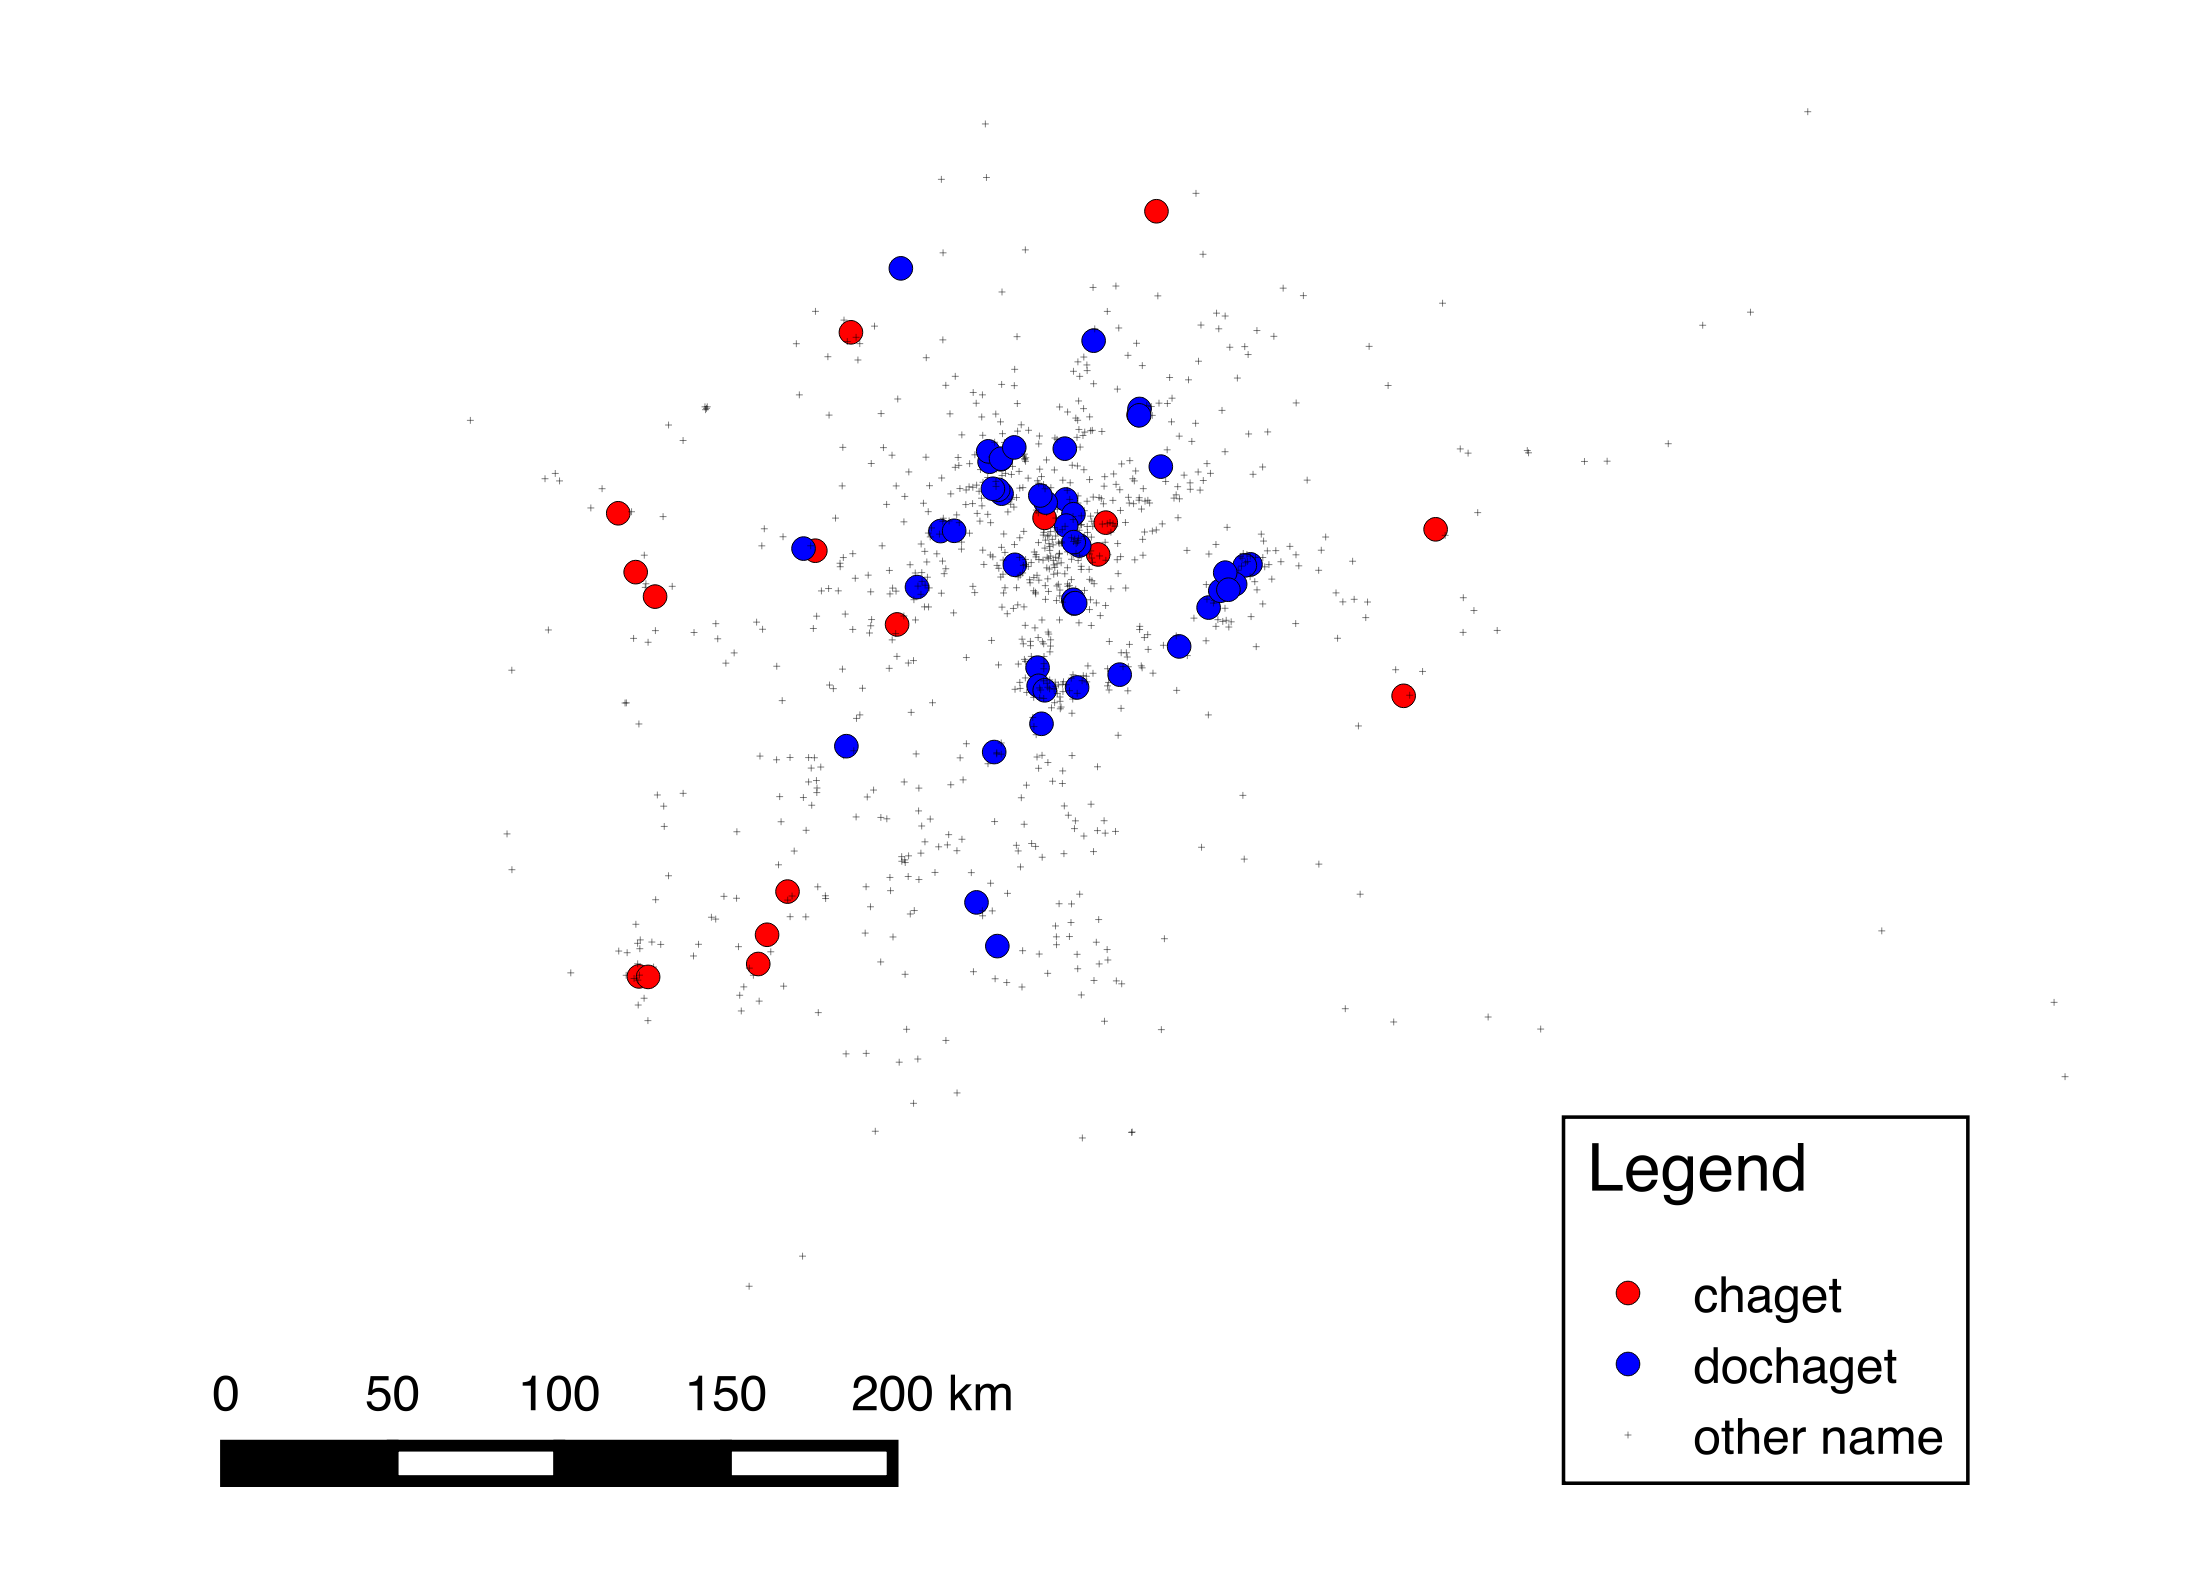
\includegraphics[width=0.9\textwidth]{figures/holton-fig1}
  \caption{Distribution of Lower Tanana names with generics \textit{chaget} and \textit{dochaget}}
  \label{holton:fig:1}
\end{figure}

There are even several instances of river mouth names which make use of a third form of the generic, \textit{khwdochaget}, a complex form including both the areal prefix \textit{khw-} and the \textit{do-} `orifice’ prefix. Consider the possibilities for a name based on the specific term \textit{Teyeddha’} and a generic ‘river mouth’. Since there are three different ways of expressing ‘river mouth’, there are at least three possibilities for this name. In fact there are even more possibilities, because the specific term can be either \textit{Teyeddha'}, which is the specific occurring in the name of the stream \textit{Teyeddha' No'}, or else the name of the stream itself can be used as the specific from which the river mouth name is derived. the choice between whether the ‘river mouth’ generic substitutes for \textit{no’}  or is added to it doubles the number of possible names to six, as shown in \ref{holton:ex:chaget}. However,  only the final name \textit{Teyeddha' No' Khwdochaget} is attested, including both the generic \textit{no’} ‘river’ from the stream name and the generic \textit{khwdochaget}.



\begin{exe}
\ex Possible generative names based on the specific term \textit{Teyeddha’ (No')} and  generic `river mouth’ terms\label{holton:ex:chaget} 
\begin{xlist}
\ex \textit{*Teyeddha’ Chaget}
\ex \textit{*Teyeddha’ Dochaget}
\ex \textit{*Teyeddha’ Khwdochaget}
\ex \textit{*Teyeddha’ No’ Chaget}
\ex[*]{ \textit{*Teyeddha’ No’ Dochaget}}

\ex \textit{Teyeddha’ No’ Khwdochaget}

\end{xlist}
\end{exe}

\noindent
So even if we could predict that the name of a place located at a river mouth should be named by combining the associated specific term with a form of the generic \textit{chaget}, we would have no way of predicting whether this generic should be added on in addition to existing generics or substituted for them, nor would we know which form of \textit{chaget} to use. In sum, we could not predict the name. And of course, we would have no way of knowing whether a particular river mouth actually had a name.

\subsection{Size of  generative clusters}
As noted above, examples of clusters of names sharing a single specific term have been cited widely in research on Alaska Dene place names.  This gives the impression of a place-naming strategy which assigns specific names to certain regions and then identifies places within this region according to the appropriate landscape generic. The Ahtna cluster based on the specific term \textit{yidateni} was noted above. A example from Lower Tanana is the cluster of 11 names based on the specific \textit{troth} ‘wild potato (\textit{Hedysarum alpinum})’, shown in Table~\ref{holton:tab:troth}. This is a well-known example, as one of the names in the cluster, \textit{Troth Yeddha’}, was recently adopted by the US Board of Geographic Names as an official place name.


\begin{table}[h]
\centering
\caption{Cluster of names based on the specific \textit{troth} 'Indian potato (\textit{Hedysarum alpinum})’}\label{holton:tab:troth}
\small
\begin{tabular}{l | l}
\textbf{Name} & \textbf{literal translation}\\\hline
\textit{Troth Yeddha'} &
Indian potato ridge\\
\textit{Troth Yeddha' No'} &
Indian potato ridge stream\\
\textit{Troth Yeddha' No' Dochaget} &
Indian potato ridge stream mouth\\
\textit{Troth Yeddha' No' Khwyighilenhde} &
where current flows into Indian potato ridge stream\\
\textit{Troth Bena'} &
Indian potato lake \\
\textit{Tr'ekhwghodegi Troth Yeddha Bena'} &
upper Indian potato lake\\
\textit{Tr'ekhwghotthidi Troth Yeddha' Bena'} &
lowland Indian potato lake\\
\textit{Tr'ekhwghotthidi Troth Yeddha' Bena' Edileni} &
flows into lowland Indian potato lake\\
\textit{Tr'ekhwghotthidi Troth Yeddha' Bena' No'} &
lowland Indian potato lake stream\\
\textit{Troth Ghotthit} &
toward the water from Indian potato\\
\textit{Troth K’eti} &
among the Indian potatoes\\
\end{tabular}
\end{table}

The cluster based on \textit{troth} in Table~\ref{holton:tab:troth} rather large, but as it turns out it is also highly exceptional. In fact, in our survey of the Lower Tanana place names data this is the largest cluster which occurs. In fact, while generativity is an important place naming strategy, as shown in Figure~\ref{holton:fig:2} the majority of Lower Tanana names---66\%---do not occur in generative clusters. Of those names which do occur in generative clusters, 54\% occur in clusters of just two names. This constitutes 69\% of the 234 generative place name clusters identified in Lower Tanana. Elaborate generative naming patterns with clusters of five or more names are extremely rare. So while the cluster based on \textit{troth} may provide a striking example of generative naming in Lower Tanana, it is far from typical.


\begin{figure}[h]
  \centering
  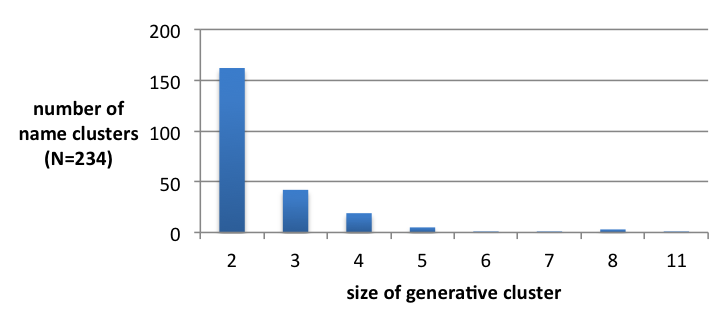
\includegraphics[width=0.9\textwidth]{figures/holton-fig2}
  \caption{Generativity of place names (number of clusters by size of cluster)}
  \label{holton:fig:2}
\end{figure}


Since the most common type of cluster is the cluster containing just two names, it is worth looking at these in more detail. Figure~\ref{holton:fig:3} breaks down the names occurring in clusters of two according to the generic term they occur with. The column labeled “none” refers to names containing no identifiable generic term. 21\% of the 324 names occurring in clusters of two. In addition, some 37\% of these names make use of the generic \textit{no’} ‘stream’; while another 24\% make use of the generic \textit{mena’} ‘lake’. Together names with these two generics and the names lacking a generic account for fully 92\% of the names occurring in clusters of size two.



\begin{figure}[h]
  \centering
  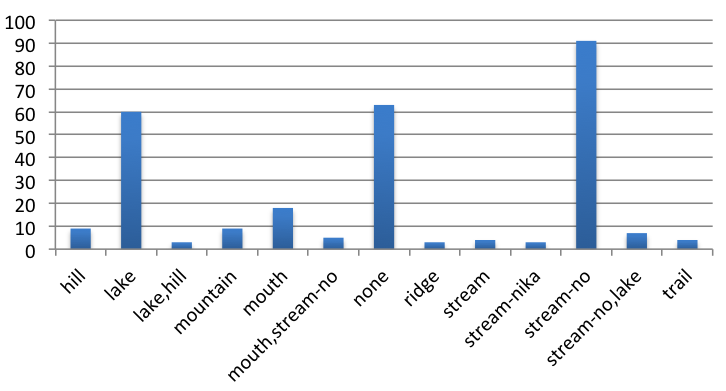
\includegraphics[width=0.9\textwidth]{figures/holton-fig3}
  \caption{Distribution of generative clusters of size=2 by type of generic}
  \label{holton:fig:3}
\end{figure}

What this means is that the primary use of the generative naming strategy is to name an associated stream or lake using the same specific term. Viewed in this context the Lower Tanana generative naming strategy seems a lot less exotic than would appear from the \textit{troth} example in Table~\ref{holton:tab:troth}. Indeed, the well-know language English frequently makes use of this strategy in naming rivers and lakes.

Generative clusters must by definition be geographically contiguous. It makes no sense to speak of two names which happen to share a specific term but are not other geographically related as being a cluster. However, there are many examples  of such non-clusters with shared specific term in Lower Tanana. The name \textit{Deba Ddhela’} and \textit{Deba No’}  share the generic \textit{deba} ‘sheep’ but are located more than 100 km from each other. Often additional qualifying material will be found in the specific term so that seeming clusters do not actually share the same generic. For example, there are two names based on the specific \textit{bezreya’} ‘land otter’, which do not cluster together. There are two additional names based on the specific \textit{bezreya’ toteth}  ‘land otter portage’; these names do cluster together, though not with the other two names based on \textit{bezreya’}. One could instead interpret \textit{toteth} ‘portage’ as a generic, in which case it might be possible to argue that names based on \textit{bezreya’ toteth}  and those based on just \textit{bezreya’} should be clustered together, but in this case the proposal fails on geographic criteria. Nevertheless, the issue of whether a particular component of a name should be treated as a specific or a generic remains. For this study we have limited ourselves to the standard set of generics outlined by \citet{kari2008}.

\subsection{Duplication of names}
\todo{not sure this section is necessary?}
It is often assumed that Dene languages avoid duplication of place names, and indeed, our study of Lower Tanana confirms that duplicate names are rare. However, the fact that names based on a single specific do not necessarily cluster together raises the possibility of name duplication, and indeed duplicate names do exist. Methodologically, the identification of duplicate names based on published sources is complicated in part by orthographic issues, as listed in Table~\ref{holton:tab:orthographic}.

\begin{table}[h]
	\centering%\small
\caption{Orthographic issues complicating the identification of duplicate names}\label{holton:tab:orthographic}
\begin{tabular}{l | l }
\textbf{Issue} & \textbf{Example} \\
\hline
vowel of possessive suffix can be represented as \textit{–e’} or \textit{–a’} & \makecell{\textit{Noghwya Bena’} \\ \textit{Noghwya Bene’} \vspace{5pt} }\\ 
%\hline
labial approximant may be represented as \textit{b}  or \textit{m} & \makecell{ \textit{Ts’oneye Bene’} \\ \textit{Ts’oneye Mene’}  \vspace{5pt}  } \\
%\hline
locative generic may be written \textit{de} or \textit{denh} & \makecell{ \textit{Nonudalyode} \\ \textit{Nonudalyodenh}\vspace{5pt} }\\
%\hline
word segmentation may vary & \makecell{ \textit{Teyh Yidatltoni} \\ \textit{Teyh Yi Datltoni} \vspace{5pt} } \\
%\hline
possessive morphology (glottal stop suffix) may be absent & \makecell{ \vspace{5pt}\textit{Khwdega’ Mena’} \\ \textit{Khwdega Mena’} \vspace{5pt}} \\

\end{tabular}
\end{table}

In order to assess to degree of name duplication in Lower Tanana we normalized the dataset to eliminate purely orthographic variation. Having done this we find that 88\% of the Lower Tanana names are unique, while another 8\% of the names occurs as doublets with exactly two duplicates (40 distinct names denoting 80 places). The remaining 4\% of names are duplicated more than twice (10 distinct names denoting 38 places). These 10 names with multiple duplicates are listed in Table~\ref{holton:tab:duplicates}.


\begin{table}[h]
\centering
\caption{Duplicated names showing number of tokens of each}\label{holton:tab:duplicates}
\begin{tabular}{l | l | c} 
\textbf{Name} &  \textbf{Literal translation} & \textbf{Tokens} \\\hline
\textit{Tobo Bena’} &
swan lake &
 6\\
\textit{Benh Dasr Bena’} &
lake shallows lake &
 4\\
\textit{Ch’etontswkh No’} &
brown water creek &
 4\\
\textit{Sanh Tena} &
summer trail &
 4\\
\textit{Sresr No’} &
black bear creek &
 4\\
\textit{Tonełkwn’ Bena’} &
clear water lake &
 4\\
\textit{Nogeddha Kan’} &
fox den &
 3\\
\textit{Teyh Chwkh} &
big hill &
 3\\
\textit{Tr’achenhnił’ode} &
where flat extends &
 3\\
\textit{Tr’iyh Tenet} &
canoe trail &
 3\\
\end{tabular}
\end{table}

Using data from the neighboring Tanacross language \citet{holton2009c} speculated that name duplication is in complementary distribution with generative names. That is, a given specific term may be repeated only if it is not used to form clusters. For example, the Tanacross name \textit{Ch’endaag Menn’}  ‘mineral lick lake’ is duplicated five times distributed roughly evenly across Tanacross territory. The name does not occur in any generative clusters. That is, there is no ‘mineral lick mountain’, ‘mineral lick stream’, etc. In fact, the specific term \textit{ch’endaag} does not occur in any other names. On the other hand, Tanacross names which occur in generative clusters appear not to be duplicated. For example, the Tanacross specific \textit{ch’inchedl}  ‘nose’ generates a cluster of four names located in close proximity, but there are no other Tanacross names which contain this specific term.

Whether or not this hypothesis regarding the complementary distribution of duplicated and generative names holds up for Tanacross, it is clearly not valid for Lower Tanana. In Lower Tanana a duplicate name may occur as part of more than one generative cluster. For example, there are two clusters consisting of \textit{Dets’eni Mena’} ‘duck lake’ and \textit{Dets’eni Mena’ No’} ‘duck lake creek’, so both of these names are duplicated and also part of generative clusters. Further, there is no constraint that Lower Tanana duplicated names be located far apart. The two instances of \textit{Noghwya Mena’} are some 64 km apart, while the two instances of \textit{Ch’elok’wy’ Teyh}  are only 4 km apart.

\section{Place naming strategies}

While the generative capacity in Lower Tanana place-naming is significant, it fails to account for a majority of Lower Tanana names. That is, the vast majority of Lower Tanana names do not occur in generative clusters. Moreover, the generative pattern does not reliably predict either the form of a name or the existence of a name for a particular place. To gain insight into place-naming strategies we must look beyond morphology and seek information about why and how particular places came to acquire their names. This requires examining the semantics of the names. For example, a name such as \textit{K'iyh Ddheł} `birch hill', which describes a  feature of the environment, can be semantically distinguished from a name such as \textit{Ch'etebił No'} `lynx snare creek', which refers to a use or function.  

Further insight into the semantics of place names can be gained  by asking speakers why places are named and by analyzing place-naming stories. In the case of Lower Tanana, this methodology is complicated by the fact that the language and its place names are remembered by only a few elderly speakers. However, we are fortunate to be able to draw on a large body of archival recordings, including many place name interviews collected in the 1970's as part of the Alaska Native Claims Settlement Act. In these recordings  the interviewers often ask directly about why a place has the name that it has. This information must of course be treated with caution, as such direct questioning invites folk etymologies. Fortunately, in the recordings that we have reviewed, the speakers are quite conservative in their responses, hesitant to offer speculative etymologies for name with which they are unfamiliar. In many cases speakers not only know why a place was named as it is but also who named it and when. This level of intimacy with places and names provides some assurance that the explanations offered by speakers on the recordings are not colored by folk etymology. 


Based on an empirical analysis of 20 legacy recordings of place name interviews we identify five primary place naming strategies used in Lower Tanana (Table~\ref{holton:tab:strategies}). These strategies are semantically defined, and thus it can sometimes be difficult to distinguish between then. For example, a place name which translates literally as `sheep mountain' might be considered environmental, describing a feature of the environment (i.e., sheep are there), or it could be considered functional (i.e., we go there to hunt sheep). In only a small number of cases can place naming strategies be identified based solely on an analysis of the name and its literal translation, and it can be misleading to make assumptions based solely on the literal translation. A case in point from our work is the name \textit{Sresr Chaget}  ‘black bear river mouth’. This might be interpreted as a (biological) environmental name based on the animal name \textit{sresr}. However, speaker Peter John clearly indicates that this is an incidental name given because someone saw bear tracks there: “Bear, they just see the bear tracks once and they call it that way” (ANL6026a, 0:59). There is no reliable method of determining the naming strategy without input from Native speakers. 

Drawing on  the archival recordings we were able to identify a place naming strategy for 856 of the 1063 names in the list. In the following subsections we describe each of the five major strategies in more detail.

\begin{table}[h]
\centering
\caption{Major Lower Tanana place-naming strategies}\label{holton:tab:strategies}
\begin{tabular}{l | l}
\textbf{Strategy} & \textbf{Description}\\\hline
Environmental & describing the geographic, environmental, or biological features of a place\\
Incidental & recalling something that happened or was seen at a place\\
Functional & describing how a place is used (human affordance)\\
Metaphorical & describing what a place resembles\\
Personal & incorporating a personal name\\
\end{tabular}\end{table}



\begin{figure}[hb]
  \centering
  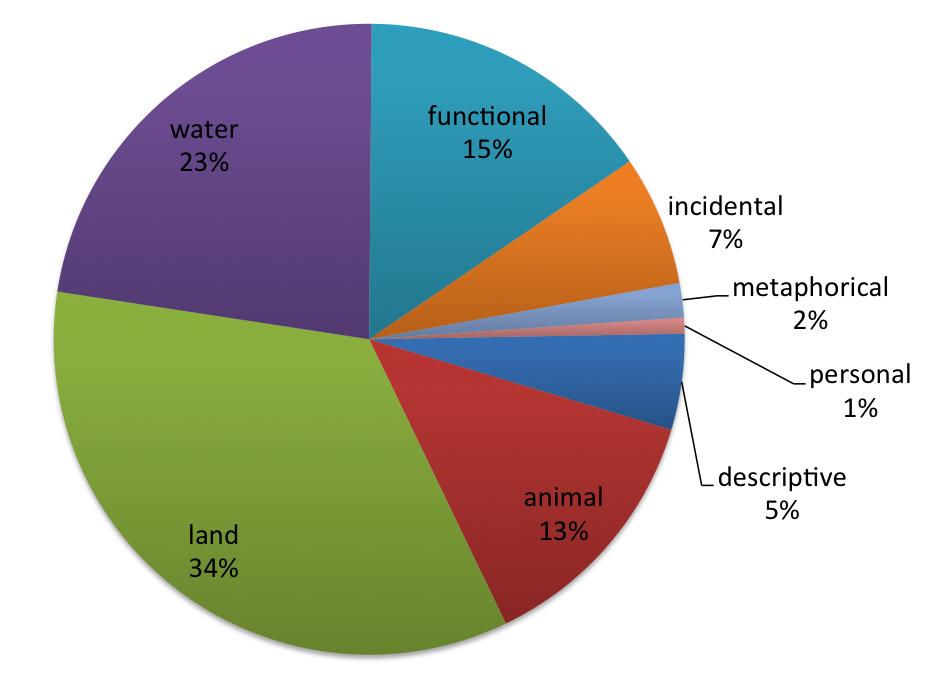
\includegraphics[width=0.6\textwidth]{figures/holton-fig4}
  \caption{Distribution of names by naming strategy \hl{Do we want to keep this pie chart?}}
  \label{holton:fig:4}
\end{figure}



\subsection{Environmental names}
We use the term \textsc{environmental} to classify place names that refer to geographic, environmental, or biological features. These features could be the size of a hill or field, the clarity of a body of water, how a river behaves in relation to the land, and what types of trees, fish, or other organisms than can be found at a location. This is a broad category within which we can identify three important subcategories: land, water, and animal. Environmental features referring to land and water dominate the Lower Tanana place naming system, accounting for more than half of the names for which a naming strategy has been identified (see Figure~\ref{holton:fig:4}). This emphasis on names which describe the environment is perhaps not unexpected given the close relationship between Lower Tanana people and their land- and waterscape. Indeed, the percentage of environmental names in Lower Tanana is comparable to that reported for Inuinnait by \citet[138]{collignon2006} and may be a significant feature of hunter-gatherer societies.

Several examples of names employing the environmental strategy are given in  Table~\ref{holton:tab:environmental}. The table lists the literal translation alongside the Lower Tanana name; however, the crucial criterion for determining that these are environmental names is verbal confirmation from speakers in the place name interviews. We avoided classifying names as environmental unless we could find evidence of speaker confirmation. One important caveat of this approach is that it does not account for potential tendency of a speaker to offer folk etymologies. Dene names are largely morphology transparent, so speakers have ready access to their literal meanings and could easily draw on this (consciously or not) in order to provide an environmental interpretation. Significantly, speakers do not consistently draw on the literal translation when providing an explanation for a name. As we shall see in the discussion of incidental names in the following section, in some cases speakers insist that the literal translation does not simply characterize the place but rather refers to a specific incident. As noted above, \textit{Sresr Chaget} ‘black bear river mouth’ is not a place with black bears but rather a place where a specific incident involving black bears occurred. In other words, speakers often know why places were named, and this topogenesis is a part of the knowledge of the name, obviating the need for a folk etymology.


\begin{table}[!h]
\caption{Names using the Environmental strategy}\label{holton:tab:environmental}
\begin{tabular}{L{3.5cm} | L{3cm} | L{3cm} | l} 
\small
{\bfseries Name} &
{\bfseries Literal Translation} &
{\bfseries Speaker Description} &
{\bfseries Recording}\\\hline

 \textit{K’iyh} \textit{Ttha} \textit{Nilani} &
‘the one with the young birch’ &
young birch &
0985b \\
 \textit{Tonełkwn’ Mena}’ &
‘clear water lake’ &
clear water; clear lake &
0987a; 0988a \\
 \textit{Chenh} \textit{Chwkh} &
‘big meadow’ &
big open flat with no trees on it &
0991a\\
\textit{Tu} \textit{Nadełdenh} &
‘where there is hot water’ &
hot water &
0989b \\
\textit{K’wy}’ \textit{Ch’eda}’ &
‘tough willow’ &
lake with willows on the side &
0989b; 6026b\\
 \textit{Nudh’onh} \textit{Mena}’ &
‘island is there lake’ &
island lake &
0984a\\
\textit{Beghentadhdleni} &
‘current flows behind  it’ &
the bend behind the hill &
0987b \\
\textit{The’odi} &
‘all the time’ &
you hear noise all the time, from the wind &
0984b

\\
\textit{Ch’enok’et} &
‘mineral lick’ &
moose lick salt there &
0985b \\
 \textit{Menh} \textit{K’wkhchwkh} &
‘on big lake’ &
big lake &
0988a \\
\textit{Dwkh} \textit{T’wkhde} &
‘elevated nest place’ &
nests in the tree &
0989a; 6018a\\
\textit{Khwtrela} &
‘moist place’ &
means wet &
0988a \\
\textit{T’egeth Yozra Nilani} &
‘cotton tree hill’ &
\textit{t’egheth yozra} means cotton tree; young cotton trees &
0984b; 6026a\\
\textit{K’wy’ Zrusr Yi Mena’} &
‘willow lake’ &
willow lake &
0984b\\
\textit{Thakwtadhlenh No’} &
‘ripple creek’ &
water running over rocks &
0984b \\
\textit{Ts’eba Nu’} &
‘spruce tree island’ &
speaker confirms spruce tree island &
0984b\\
\textit{K’iyh Tretr Ch’oghwna’} &
‘dry birch ridge’ &
birch on the ridge &
0987b\\
 \textit{Tr’ekhodetthatlde}  &
‘where it got chopped out’ &
they made a creek through there &
0987b\\
\textit{Łeyeth Toteth} &
‘dwarf birch portage’ &
little short willow &
0985b\\
\textit{Teyh Yitodaghi’odenh} &
‘slough extends into hill’ &
lake going in between the hill &
0987a\\
\end{tabular}
\end{table}

There is some danger of over-interpretation with environmental names. In particular, it is sometimes the case that environmental names don’t actually refer to existing geographic features. For example, the name \textit{Batr’a Ch’ilanh Teya’} means literally ‘obsidian is there hill’, but when questioned about the name, speaker Peter John is insistent that there is no obsidian on this hill. “No rocks there; they just named it like that. They only one that’s there is the little island.” (ANLC0989a, 00:26, 1975-05-25). The mere fact that a name describes an environmental feature does not necessarily imply that the name was given because of that description. Or it may be the case that speakers no longer have knowledge of the environmental features for which the place was named.

\subsection{Incidental names}
A small but significant portion of the Lower Tanana names refer not to the environment but to an event which occurred at the location named. We use the term \textsc{incidental} to denote a naming strategy that describes a event that occurred at a place or something that was observed at a place \citep[cf.][]{goehring1990}. Incidental names are not particularly frequent in the Lower Tanana corpus, comprising a mere 7\% of names, but they play a particularly important role in providing an historical connection to the landscape. The significance of incidental names cannot be directly inferred from the name itself or its literal translation. Rather, the name serves a sign which indexes an historical event. Knowledge of this event is an essential part of knowledge of the name. Of course, the names could be used and referred to without be aware of the associated event, but speakers repeatedly emphasize that knowledge of the associated event is a crucial part of knowing the name.

Some examples of incidental names are given in Table~\ref{holton:tab:incidental}. In some cases incidental names vividly describe the associated event, as with the name literally translated as ‘where a brown bear knocked someone down’. In other cases the associated event is more or less opaque, as with the name literally translated as ‘rabbit potlatch house’. These more opaque names “make sense” once you know the story of the event behind them, but there is no way to infer knowledge of the event from simply knowing the name itself.


\begin{table}[htb]
\caption{Names using the Incidental strategy}
\label{holton:tab:incidental}
\small
\begin{tabular}{l | L{3cm} | L{3cm} | l}
{\bfseries Name} &
{\bfseries Literal Translation} &
{\bfseries Speaker Description} &
{\bfseries Recording}\\\hline
\textit{Sresr Chaget} &
‘black bear mouth’ &
named so because they saw a set of bear tracks there once &
6018a\\
 \textit{Gwkh} \textit{Nitsił} &
‘rabbit potlatch house’ &
name comes from seeing one set of rabbit tracks &
6026b\\
\textit{Tsugi Tl’wgha’} &
‘marten’s grass’ &
caught a marten there &
0992a\\
 \textit{Dathdlazri Dena’iłghełdenh} &
‘where a brown bear knocked someone down’ &
a brown bear knocked us down &
0991b\\
\textit{Nu K’ech’idet’otthde} &
‘place where island is cut in two’ &
someone sliced island in two &
0985a\\
\textit{Tsoni} \textit{Tr’iłtanh} \textit{No}’ &
‘creek where we found a brown bear’ &
place where we saw a dead bear &
0991b\\
\textit{Dedenach’ilok} &
‘someone hurt us’ &
brown bear killed a man &
0987b\\
\textit{Dzak Todhyodenh} &
‘where Jack came’ &
First time they saw a white man at that place. His name was Jack. &
0987a\\
\textit{Ch’edhatr’eghikanh Nunkw} &
‘person got caught paddling doing something they’re not supposed to’ &
person got caught there and they killed him &
0988a \\
\end{tabular}
\end{table}

Speakers’ descriptions of incidental names may be quite vivid, reflecting the fact that such names are often embedded within a larger shared cultural memory. Regarding the name \textit{Dedenach’ilok} Peter John’s explanation is much more detailed than the literal translation ‘someone hurt us’ would indicate. John notes that a “brown bear killed a man right there” (ANLC0987b, 45:07). In some cases incidental names verge on the mythological, though speakers do not construe them as such. For example, in describing the name which translates literally as ‘place where island is cut in two’ Peter John says that {\textquotedbl}somebody got jealous and tried to fight with his wife, and he missed her with a knife{\textquotedbl} (ANLC0985a, 17:07). The implication here is that the physical separation in the island is a direct result of the knife cutting through the island after it missed its intended target.

It can sometimes be difficult to distinguish the incidental strategy from the environmental and functional strategies. The name \textit{Noghwya Ch’edonhden} means literally ‘where a frog had supper’. In our data speakers offered no further explanation for the name, so the strategy being used is unclear. If the place was home to many frogs, or even many flies for frogs to eat, it could be considered to be using the environmental strategy. However, it is equally possible that somebody once saw a frog eating there and named the place so, which would then be use of the incidental strategy. Without further consultation of a native speaker, the strategy will remain a mystery. Similarly, the name \textit{Gwkh} \textit{Nitsił} ‘rabbit potlatch house’ could be seen as a functional because the place functioned as a potlatch site. However, speakers insist that the place was named based on one instance of seeing rabbit tracks at this location, indicating that the incidental strategy is being used.

\subsection{Functional names}
We use the term \textsc{functional} to denote names which refer to how the places they denote are used. Functional names have a direct relevance to ecosystem services, since they describe the way humans relate to the land, or what \citet{levinson2008} calls human affordance. Places named for the use of animal snares or fish traps, graveyards or gravesites, and places that can be used to gather resources fall under this category. Functional names comprise 15\% of the Lower Tanana names. It could be argued that names for lakes and rivers that include the type of fish found there could be classified as ‘functional’, because one could speculate the lake would be used to catch that type of fish. But, for the purpose of this project, without the speaker expressly saying that is why the place was named, they will remain under the ‘descriptive’ category. Examples of the ‘functional’ strategy at work are shown in Table~\ref{holton:tab:functional}.


\begin{table}[htb]
\caption{Names using the Functional strategy}
\label{holton:tab:functional}
\small
\begin{tabular}{L{3.5cm} | L{3cm} | L{3cm} | l}
{\bfseries Name} &
{\bfseries Literal Translation} &
{\bfseries Speaker Description} &
{\bfseries Recording}\\\hline

 \textit{Ch’etebił} \textit{No’} &
‘lynx snare creek’ &
\textit{Ch’etebił} is an old name for a lynx snare &
6017a\\
\textit{Khwn’a Khwjeda’}  &
‘rotten river’ &
easy place to get lost &
0987a\\
 \textit{Niłk’ach’enidetl’unh} \textit{Mena}’ &
‘snares set on both sides lake’ &
means snares on both side &
0985b\\
 \textit{Bek’et} \textit{Notr’iyhtr’edełgoyi} &
‘on it we dry out a canoe’ &
we dry canoe on there &
0991b\\
 \textit{Nełtrith} \textit{Hał} \textit{Toteth} &
‘wolverine trap portage’ &
wolverine portage &
0985b\\
\textit{Ninotr’iyhleyahdenh} &
‘where canoes are left’ &
where they leave canoe to climb the hill &
0985b \\
 \textit{Bek’et} \textit{Tabił} \textit{K’at} \textit{Khwloyh} \textit{Mena}’ &
‘net places are on it lake’ &
where they used to set nets &
0987a\\
 \textit{Be’ot} \textit{Noyeghiłdhedenh} \textit{Tth’enhk’at} &
‘the grave of the one that was killed by his wife’ &
A woman killed her husband and that man was buried there &
0987b; 6026b\\
 \textit{Beghw} \textit{Tr’etreghi} &
‘by it we cry’ &
Lot of people used to go there and cry. Used to be village there with a big gravesite &
6030a\\
 \textit{Dwkhtso} \textit{Dedhlodenh} &
‘where there are caches’ &
cache is there, above the ground &
0989a\\
\textit{K’oł Tr’uneyh Ddhela’} &
‘we obtain whetstone mountain’ &
we pick stones for sharp knife or arrowhead (\textit{k’oł} `sharpening stone') &
0991b; 6026b; 6026a\\
\end{tabular}
\end{table}


Functional names share with incidental names an inherent human connection to the landscape, but whereas incidental names evoke a particular historical event, functional names refer to a continuing relationship with a place. In some cases the nature of this relationship is clear from the semantics of the name, but the meaning of other functional names is more opaque. For example, \textit{Khwn’a Khwjeda’} means literally ‘rotten river’, but in order to know why this river is considered rotten one must know more about the place and why it was named. Peter John explains that this place was named “because they got so many islands. There’s nothing but islands up there. They’re easy to get lost in.” (ANLC0987a, 45:09).

\subsection{Metaphorical names}
We use the term \textsc{metaphorical} to denote the naming strategy that uses metaphor to describe what a place resembles. This category is similar to what \citet[132]{collignon2006} calls morphological analogy. The metaphorical strategy is essentially a type of environmental naming strategy in that it makes reference to the appearance of a feature, but in using analogy metaphorical names reflect a greater degree of human interaction with the landscape. This is a rather small category; we identified only 15 names which use the metaphorical strategy, some of which are listed in the Table~\ref{holton:tab:metaphorical}.


\begin{table}[ht]
\caption{Names using the Metaphorical strategy}
\label{holton:tab:metaphorical}
\small
\begin{tabular}{L{3.5cm} | L{3cm} | L{3cm} | l}
{\bfseries Name} &
{\bfseries Literal Translation} &
{\bfseries Speaker Description} &
{\bfseries Recording}\\\hline

\textit{Tr’edhdo} &
‘someone is sitting’ &
rock formation looks like someone sitting down &
0987b\\
 \textit{Sresr} \textit{Yona}’ \textit{Tr’eghił’odenh} &
‘ram object extends out’ &
there are white rocks lined up that look like sheep walking &
6030a\\
 \textit{Seyatth’ena} \textit{No}’ &
‘my jawbone creek’ &
named for way it’s shaped &
0990a \\
\textit{Tr’iyh Khwt’ani} &
‘one like a canoe’ &
looks like a canoe &
0990a \\
\end{tabular}
\end{table}

Names in the Metaphorical category cannot be identified based solely on morphology and/or semantics but rely on speaker knowledge for their explication. For example, the name \textit{Tr’edhdo} means literally ‘someone is sitting’. This is the name of a long ridge north of Washington Creek (\textit{Tat’ali No’}), but the ridge is named for a particular rock formation which is located on the ridge—a rock formation which has the appearance of a seated figure (ANLC0987b, 40:45, 1979-05-24). On the other hand, some names which might at first appear metaphorical turn out to be descriptive once we consult speaker knowledge. For example, the name \textit{The’odi} translates literally as ‘all the time’, a rather ambiguous gloss for which it is tempting to provide a metaphorical interpretation. However, speakers are quite clear that this name is a reference to the observation that the wind blows all the time on this hill (ANLC0984a, 07:17). Hence, this name is not a metaphor but rather an environmental description.

\subsection{Commemorative names}
The \textsc{commemorative} naming strategy is used to classify those names which incorporate a personal name commemorating a particular person. We mention the commemorative strategy not because it is significant in Lower Tanana but rather because it is almost completely absent, found in only four names. Lower Tanana commemorative place names are not honorific, as are most English commemorative place names; rather, Lower Tanana commemorative place names refer to a place where someone does a certain activity. In this sense Lower Tanana commemorative names might be better characterized as personal names. The relationship is in some sense one of ownership, though this is ownership not in the sense of land tenure but rather in the sense of traditional use. The complete list of names using the commemorative strategy is given in Table~\ref{holton:tab:commemorative}.


\begin{table}
\caption{Names using the Commemorative strategy}
\label{holton:tab:commemorative}
\begin{tabular}{l | l | l | l} 
\small
{\bfseries Name} &
{\bfseries Literal Translation} &
{\bfseries Speaker Description} &
{\bfseries Recording}\\\hline

\textit{Sek’otl To’ Dazra’} &
‘Sek’otl To’s sandbar’ &
fish camp &
6030a\\
\textit{Doyelokh Beto’ Dazra’} &
‘Charlie Albert’s sandbar’ &
n/a &
none\\
\textit{Ywtltsetl’a Dazra’} &
‘Little Ywtl’s sandbar’ &
n/a &
none\\
 \textit{Bechots’idhił} &
‘Old Silas’ &
n/a &
none\\
\end{tabular}
\end{table}

All four of the names in Table~\ref{holton:tab:commemorative} make use of traditional Lower Tanana personal names, not modern English names which were later adopted by Dene speakers. This points to the names having an origin prior to the arrival of white settlers in the late nineteenth century. In two cases we know the corresponding English name as well. \textit{Doyelokh Beto’} is known in English as Charlie Albert, and \textit{Bechots’idhił} is known in English as Old Silas. Curiously, three of the four names include the generic \textit{dasr} ‘sandbar’ (possessed form \textit{dazra’}). We know from our corpus that at least one of these was a fish camp site; the remaining names are not discussed on the recordings. The one name without a generic, \textit{Bechots’idhił}, is said to refer to the location of a fox farm.

There is one additional place name in the corpus which incorporates a personal name: \textit{Dzak Todhyodenh} means literally ‘where Jack came’ and is known in English as Jack Hill. Speakers describe this as the place where they encountered the first White man, a man named Jack. So this name employs the Incidental strategy rather than the Commemorative strategy; it is not named after Jack but rather after the event of meeting Jack.

\section{Remaining challenges}

%\begin{itemize}
%\item Is generativity being under- or over-reported?
%\item How do we know what counts as a name if names are largely predictable?
%\item Just because we can predict what something would be named doesn’t mean it actually \textit{is} named.
%\item There \textit{is} variation in choice of generic, so less predictability than we might think.
%\end{itemize}

\subsection{What counts as a name?}

One of the greatest challenges for place names research is deciding just when something should count as a name. In some ways this problem is similar to the problem of deciding when a new term should be entered into a dictionary. Anyone can invent a way of a referring to something, but to be considered a place name such a reference should be conventionalized and broadly shared among a community of speakers. Moreover, a true place name should be stable over time. This criterion excludes ad-hoc forms of reference which are coined for particular speech event but then quickly discarded. Yet it is not always so easy to distinguish between ad-hoc and stable names. In English I might refer to the second of a series of three lakes as ‘second lake’, but when does this become a name rather than an ad-hoc reference. English provides some clues in the grammar, in that ad-hoc references to lakes are more likely to occur with an article, as in “Let’s go up to the second lake;” while names for lakes in English tend to occur without articles, as in “Let’s go up to Second Lake.” However, this criterion does not work with all English place names. We can easily speak of the Yukon River and the Lower Yukon River. The former is clearly a name, but the status of the latter is less clear. In any case not all languages offer such grammatical criteria for distinguishing names from ad-hoc references. In Dene languages if a stream is named \textit{Sresr No’} ‘black bear creek’, then the obvious way to refer to the lake which feeds the creek is \textit{Sresr Mena’} ‘black bear lake’ (or perhaps \textit{Sresr No' Mena'} `black bear stream lake'). Or it could just be unnamed. The fact that a name can be generated does not necessarily make it a name. The generative capacity in Dene naming is significant, but as we have seen it is not deterministic.

In particular, in spite of elaborate mechanisms for generating Dene place names, it is not the case that every form which can be generated will be a name. As noted above in the discussion of the use of the generic \textit{chaget} ‘river mouth’, naming is a deliberate practice, and speakers know what counts as a name. Thus, we must beware the tendency to over-differentiate and infer names for places which are actually unnamed. This caution is particularly relevant when working with severely endangered languages with few remaining speakers. Some existing reports may be problematic in this regard. For example, \citet{kari2012} list two lakes \textit{Khwgongw Nitl’et K’otena Mena’}  ‘upper cranberry lake’ and \textit{Khwghonhtthit Nitl’et K’otena Mena’} ‘lower cranberry lake’, distinguished by the directional terms \textit{khwgongw} ‘upland’ and \textit{khwghonhtthit} ‘lowland’. But when asked specifically about the names for these two lakes speaker Peter John was insistent that there was only one name. “The whole thing is what we call \textit{Nitl’et K’otena Mena’,} this whole thing, all this, all the lakes” (ANLC0985a, 27:37, 1979-05-24). Here we come up against differing conceptualization of the landscape. Lower Tanana assigns one name to a set of lakes, whereas as English insists on separate names for each lake. On this recording the English-speaking interviewers are clearly unhappy with Peter John’s response, since it doesn’t match their own conceptualization of the landscape.

Of course Lower Tanana speakers do have the directional terms ‘upland’ and ‘lowland’ available to them if they need to distinguish between the two lakes, but using directionals to distinguish places is not the same as naming them, any more than using upper and lower to distinguish parts of a river in English constitutes assigning a name to those parts of the river.
The key to understanding what places are named is that speakers know not only what is named but what is not named. Thus, speakers have knowledge of places which extends beyond simple inventories of names. Speakers often know what things are not named. For example, the string of islands in the Tanana River below the confluence with the Tolovana River is known as \textit{Nonudalyodenh}, literally ‘where islands extend across’. But speakers are keenly aware that only one of these islands, \textit{Khenge Nu’}, has a name; the others are known but unnamed places (ANLC0987a, 44:00).

\subsection{Optionality and variation of generic term}
In many cases speakers will freely omit the generic portion of a compound name when the referent is clear from the context, and it can be difficult to decide whether the generic is actually part of the name. This often occurs with the generic \textit{denh} ‘specific place’. Speakers will often omit the generic \textit{denh} when discussing a place. When questioned about the validity of the name \textit{Khwtethmenhdenh}, speakers explain that the name is actually \textit{Khwtethmenh} but that \textit{Khwtethmenhdenh} can be used when you’re talking to someone that doesn’t know where the place is (ANLC2556a, 2:34). Similarly, in an interview discussing the name \textit{Tr’enotokhwghiłch’ełdenh} is only pronounced with the generic \textit{denh} when introducing the name; five successive pronunciations of the name omit the generic and refer merely to that follow \textit{Tr’enotokhwghiłch’eł} (ANLC0989a). This suggests that for at least some names the generic \textit{denh} may not be a part of the place name. However, it is also possible that the name without the generic represents a clipping, similar to the way someone might use the form Everest for Mount Everest.

In some cases the historical recordings differ from the published place name list with respect to the presence of the generic. The name \textit{Dotron}’ \textit{Tr’iłtanhde} \textit{No}’ listed in Kari et al. (2012) contains two generics, \textit{de(nh)} and \textit{no’}, but in the recordings the name is consistently pronounced as \textit{Dotron}’ \textit{Tr’iłtanhde} \textit{No}’, without the generic \textit{de(nh)} (ANLC0984b)\textit{}. Similarly, the name listed as \textit{Tl’wkh Dhoydenh} in Kari et al. (2012) is consistently pronounced on the recordings without a generic as \textit{Tl’wkh Dhoy}, literally ‘grass sand’ (ANLC6026b).
There are also instances of names for which speakers vary as to the choice of generic. The name \textit{Nonudalyodenh} is also pronounced as \textit{Nonudalyokhw}, the latter form substituting the generic \textit{khw} ‘area’ for the generic \textit{denh} ‘specific place’ (ANLC0987a; ANLC0992a; ANLC6026b). It is not clear that there is any meaning difference, e.g., denoting a greater or lesser expanse. Moreover, this place can equally be referred to as \textit{Nonudalyo}, without either generic\textit{} (ANLC0992a).

An even more striking case of variation in generic term can be found in the name \textit{Mentoli No’}, literally ‘flows among lakes creek’. Peter John explains that “people used to call it two different ways, \textit{Mentoli Chaget} and \textit{Mentoli No’}” (ANLC0987a, 10:52). That is, either the generic \textit{chaget} ‘rivermouth’ or \textit{no’} ‘creek’ can be used with this name. When questioned regarding this Peter John insists that “\textit{chaget} means creek.”

\subsection{Names can change}
Names are not permanent but can change over time. In Lower Tanana the majority of the names are environmental and provide direct insight into the nature of the environment and the way humans experience the landscape. But as the environment changes the names can change too. Things that didn’t get used much didn’t get names. Places like lakes that have dried up and are no longer used, the names don’t get used. Speakers are often aware of places which used to be named but no longer have any names. Discussing a set of sloughs along the Tanana River, Peter John remarks, “Now over this way there used to be a lot of lakes over this way, and it’s all filled up with sand. And every one of them had a name, but then there’s no more lakes around there so they don’t use the name” (ANLC0988a, 26:45).

Speakers are also aware of places which used to have different names, though not all speakers necessarily remember the older names. Regarding the place known today as \textit{Dets’eni Trona’ Mena’} speaker Peter John says “That’s wrong name. It’s not \textit{Dets’eni Trona’ Mena’}. They just call it that. The young people right now today. But you go back one hundred years ago it’s \textit{Ts’u T’okh Mena’}…. That’s the old time way. \textit{Dets’eni Trona’ Mena’} that’s just the young people name that.” (ANLC0987a, 41:26). The newer name appears to be a calque of the unofficial English name Duckshit Lake. Some old names are still remembered centuries after they have ceased to be used. “\textit{Bedzeyh T’okh No’}, that’s the name of the Murphy Dome. Now, this is about 200 years ago. Now, after that, we call it \textit{Ts’etseye Bek’et Khenitighi’oyi}. After that, they say Murphy Dome.” (ANLC6026b, 18:45).

%names change (or disappear) because people stop using them (ANLC0988a, 26:34)
%Names can be transferred to another site. \hl{EXAMPLE}.

\section{Conclusion: Places get named for a reason}

Our study place of naming strategies in Lower Tanana reveals that the generative naming pattern is much less prominent than has been reported for other Alaska Dene languages. The vast majority of Lower Tanana place name clusters sharing a common specific term contain just two names. The often-cited clusters of multiple names generated by combining a single generic with multiple different generic terms are extremely rare. We have documented only six clusters of Lower Tanana names containing six of more names. In practice, Lower Tanana place naming is much less deterministic. A more economical explanation for the preponderance of the specific + generic naming pattern is the prevalence of the environmental naming strategy. More than half of Lower Tanana names describe environmental features referring to land or water. Given this tendency it is natural that many names incorporate landscape or waterscape generic terms.

The attractiveness of the generative hypothesis may be due to the analyzability of Dene place names. In his study of Ahtna places names, Kari notes that “...it is striking that 89\% of the names are fully analyzable” \citeyearpar[200]{kari2010}. However, this figure may actually be typical of morphologically complex languages. For example, \citet[103]{collignon2006} reports that fully 97\% of Inuinnait names are analyzable, and  \citet[78]{goehring1990} concludes that “in all cases save one the Inuktitut names are clearly translatable within the local context of the physical appearance or some aspect of human lived experience.” That is not to say that Dene and Inuktitut place-naming strategies are equivalent (in fact, they are quite different; see \citealt{holton2018b}); but the complex morphology exhibit in languages like Dene may lead us to view the generative strategy as more productive than it actually is. 




In the end, places get named not because a name can be generated but rather because of a conscious need to name a place. In other words, while a generative theory of place-naming in Lower Tanana can provide a post-hoc explanation for binomial names containing landscape generics, it has limited predictive value. For example, given the name for a certain creek we cannot predict that the name of a nearby lake will incorporate the same specific term. In fact, we cannot predict that the lake will even have a name. If the lake is named and does incorporate the same specific name as the creek, then we can posit a generative explanation. If not, then the generative theory fails. Indeed, we must consider the possibility that the so-called generative strategy may be epiphenomenal, existing only as a convenient post-hoc grouping of names which share a specific term.

What a generative theory of place naming fails to capture is that places get named for a reason. We have discussed some the Lower Tanana naming strategies above, but in each case the choice to deploy that strategy is deliberate. Place names provide a reference point for human interaction with the landscape. As Peter John remarks in the epigraph above, “People used to name these things as they see them” (ANLC0992a, 01:10). These attitudes toward place naming evidenced by Peter John and other speakers  in the Lower Tanana recordings are in fact similar to those reported for other Alaska Dene languages. Referring to Dena’ina names \citet[15]{evanoff2010} says “The place is named something special; you’ve been there, it’s named because it has to be passed on and it’s about something that was done there.... Everywhere you go it brings back memories of what happened there.” To quote Peter John once more, “The ones that they used more is the ones that got named.” (ANLC0988a, 26:34)


%As scholars from \citet{boas1934} to  \citet{basso1988} have repeatedly emphasized, names are not mere abstractions on the landscape. Rather, place names reflect speakers’ conceptualizations of the landscape and tell us something about how speakers relate to the land. That said, speakers do not have complete freedom when assigning names: place names are constrained by syntactic rules and by conventional patterns of naming. Speakers make use of language-specific place-naming strategies to create names. Most languages draw on multiple naming strategies. For example, English makes use of both a commemorative strategy (e.g., Mt. McKinley) and a resource-based strategy (e.g., Salmon Creek). Within Dene languages one strategy has received considerable attention in the literature.

As scholars from \citet{boas1934} to  \citet{basso1988} have repeatedly emphasized, names are not mere abstractions on the landscape. Rather, place names reflect speakers’ conceptualizations of the landscape and tell us something about how speakers relate to the land. Although this study of Lower Tanana place naming strategies is preliminary, our work shows the power of using archival recordings in order to understand Dene naming strategies. To date most work on Alaska Dene place names has focused on generating name inventories or on assembling travel narratives which cite place names as waypoints \citep[e.g.,][]{kari2010}. The groundbreaking work of \citet{kari1996a} to correlate the distribution of names with the morphological structure of those names reveals how a large place name database can support geographic analyses. By including archival recordings as well, we are able to examine not only morphology but also speaker knowledge of names---knowledge which is not necessarily recorded in the place name lists and cannot always be inferred from the morphology or semantics of the names. As access to place name inventories and archival recordings increases we can look forward to additional insights into Alaska Dene place-naming strategies and a better understanding of the complex relationship between Dene people and the land.

\refheading
\bibliographystyle{ldc}
\bibliography{holton}

\orcidfooter{Gary Holton}{holton@hawaii.edu}{0000-0002-9346-1572}
\orcidfooter{David Jason Harris}{djharris2@alaska.edu}{}

\label{holton-ch-end}
